\section{OMPAS : RAE guided by planning (9 min)}
\begin{frame}{A new RAE implementation}

    Assets:
    \begin{itemize}
        \pause
        \item Handle concurrency inside methods
        \pause
        \item Refinement guided by an HTN temporal planner
        \pause
        \item Custom Acting language to define acting domains
    \end{itemize}

\pause
\begin{center}
    \begin{tikzpicture}%[scale=0.6, every node/.style={scale=0.6}]
        \node[draw = black, very thick,
            minimum width = 10em,
            minimum height = 3em,
            rounded corners,
            text = black,
            text centered, text depth = 5em,
            align = center,
            ] (R) at (0,0) {RAE};
  
            \node[draw = black, very thick,
            text centered,
            rounded corners,
            text = black,
            align = center,] (M) at (-1,-0.25) {Main \\\small Agenda};
  
  
            \node[draw = black, very thick,
            text centered,
            rounded corners,
            text = black,
            align = center,] (S) at (1,0.25) {Select};
  
            
            \node[draw = black, very thick,
            text centered,
            rounded corners,
            text = black,
            align = center,] (P) at (1,-0.75) {Planner};
  
            \path[->, every node/.style={font=\sffamily\small}]
            (M) edge[bend left] (S)
            (S) edge[bend right] (P)
            (S) edge[bend left] (M)
            (P) edge[bend right] (S);
  
            
  
  
        \node[draw = black, very thick,
            text centered,
            left = 5em of R,
            minimum width = 4em,
            minimum height = 3em,
            rounded corners,
            text = black] (Mon) {Monitor};
        
        \node[draw = black, very thick,
            text centered,
            right = 6em of R,
            minimum width = 4em,
            minimum height = 3em,
            rounded corners,
            text = black] (Pl) {Platform};
        
        %text between Monitor and RAE
        \path[->]
        (Mon.20) edge[bend left] node [midway, above, align=center] {\footnotesize \textit{Tasks}} (R.170)
        (R.-170) edge [bend left] node [midway, below] {\footnotesize \textit{Internal State}} (Mon.-20)
    
        (R.10) edge[bend left] node [midway, above] {\footnotesize \textit{Actions}} (Pl.160)
        
        (Pl.-160) edge [bend left] node [midway, below, align = center] {\footnotesize \textit{Platform State},\\\footnotesize \textit{Action Status}} (R.-10);
        
        \node[text centered,
            below = 2em of Mon,
            minimum width = 5em,
            minimum height = 3em,
            text = black,
            align =center] (H) {\footnotesize Human,\\\footnotesize Program};
        \draw[-latex] (H)--(Mon);
    \end{tikzpicture}

\end{center}

\end{frame}

\begin{frame}{Improve high-level choices by anticipating RAE choices in function of the agent behavior}

    Improve Select $\rightarrow$ method selection based on:
    \begin{itemize}
        \pause
        \item applicability $\rightarrow$ pre-conditions($\xi$)
        \pause
        \item future choices \textbf{(instantiating, refinement)}
        \pause
        $\rightarrow$ embedded in operational models
        \item primitives tasks outcome $\rightarrow$ platform model
    \end{itemize}

\end{frame}
\begin{frame}[fragile]{Extend Select with the call of a planner}
    \begin{columns}[c]
        \begin{column}{0.4\textwidth}
            \begin{algorithm}[H]
                \begin{algorithmic}
                    \scriptsize
                    \Function{Select}{$\tau$}
                    \State $m \gets \varnothing$
                    \State $\xi$ $\gets$ \Call{Get-State}{}
                    \State $M$ $\gets$ \Call{Applicable}{$\tau$, $\xi$} $\setminus$ \Call{Tried}{$\tau$}
                    
                    \State \Return \textbf{arbitrary} $m \in M$ \label{line:return-failure}
                    
                    \EndFunction
              
                \end{algorithmic}
                \caption{Greedy select for a task $\tau$.}
                \label{alg:plan}
              \end{algorithm}
        \end{column}
        \pause
        \begin{column}[c]{0.1\textwidth}
            \centering
            $\rightarrow$
        \end{column}
        
        \begin{column}{0.55\textwidth}
            
            \begin{algorithm}[H]
                \begin{algorithmic}
                    \scriptsize
                    \Function{PlanSelectMethod}{$\tau$}
                    \State $m \gets \varnothing$
                    \State $\xi$ $\gets$ \Call{Get-State}{}
                    \State $M$ $\gets$ \Call{Applicable}{$\tau$, $\xi$} $\setminus$ \Call{Tried}{$\tau$}
                    \State $\pi$ $\gets$ \Call{Get-Parent-Plan}{$\tau$} \label{line:get-parent-plan}
                    \If{$\pi = \varnothing$\textbf{ or not } \Call{Is-Valid}{$\pi$}} \label{line:check-valid}
                      \State $\pi \gets$ \Call{Call-Planner}{$\tau$, $\xi$} \label{line:call-planner}
                      
                    \EndIf
                    \State $m$ $\gets$ \Call{Get-Method-From-Plan}{$\pi$, $\tau$} \label{line:get-method}
                    \If{$m \neq \varnothing \land m \in M$} 
                      \State \Return $m$ \label{line:return-success}
                    \Else
                      \State \Return \textbf{arbitrary} $m \in M$ \label{line:return-failure}
                    \EndIf
                    \EndFunction
              
                \end{algorithmic}
                \caption{Plan-based method selection for a task $\tau$.}
                \label{alg:plan}
              \end{algorithm}
        \end{column}
    \end{columns}
\end{frame}

\begin{frame}{Input and output of the planner}


    \begin{tikzpicture}[thick,scale=0.8, every node/.style={scale=0.8}]
        \node[draw = black, very thick,
            text centered,
            minimum width = 12em,
            minimum height = 5em,
            rounded corners,
            text = black,
            align=center] (F) at (0,0) {\textbf{Planner}\\$P_\Delta$};
        \node[above=1em of F, xshift = -12em] (t1) {\Large\textbf{Inputs}};
        \node[above=1em of F, xshift = 12em] (t2) {\Large \textbf{Outputs}};
        \node[yshift = 1.5em, xshift = -12em] (t3) {\textbf{State, Task instance}};
        \node[yshift = -1.5em, xshift = -12em] (t4) {\textbf{$P_\Delta$}};
        \draw[-latex, ultra thick] (-6,0)--(F.west);
        \node[xshift = 15em] (t5) {\textbf{Hierarchical Plan}};
        \node[below=3em of t5, align = center] (t6) {Methods for every tasks\\
        Actions ordering};
        \node[below=2em of t4, align =left] (t7) {Descriptive models of:\\
        - Abstract tasks and methods \\
        - State-functions\\
        - Primitive tasks };
        \path[->] (t4) edge (t7)
        (t5) edge (t6);
        \draw[-latex, ultra thick] (F.east) -- (t5);
    \end{tikzpicture}

\end{frame}


\lstset{basicstyle=\tiny, columns=fullflexible}




\begin{frame}{Scheme OMPAS : An acting language...}
    Acting primitives:
\begin{itemize}
\pause
    \item exec-task: execute and monitor a task
\pause
    \begin{itemize}
        \item primitive-task: request to the platform
        \item abstract-task: select a method and execute the operational model.
    \end{itemize}
\pause
    \item read-state: return the value of a state-variable
\end{itemize}
\end{frame}

\begin{frame}[fragile]{...to define acting domains $A_\Delta$...}
    \setlength{\leftmargini}{0pt}
    \begin{columns}
        \begin{column}{0.5\textwidth}
            High-level primitives:
            \begin{itemize}
                \footnotesize
                \item Task (label, typed parameters):
                \tiny
                \begin{lstlisting}
(def-task t_process_package
    '(?p package))
                \end{lstlisting}
                \footnotesize
                \pause
                \item Method (label, typed parameters, pre-conditions, body):
                \tiny
                \begin{lstlisting}
(def-method m_process_to_do_r
'((:task t_process_package)
  (:params (?p package))
  (:pre-conditions
    (!= (package.processes_list ?p)
        nil)))
  (:body
    (do
     (define ?m ...)
     (t_process_on_machine ?p ?m)
     (t_process_package ?p)))))    
                \end{lstlisting}
            \end{itemize}
        \end{column}
\pause
        \begin{column}{0.5\textwidth}
            Low-level primitives:
            \begin{itemize}
                \pause
            \footnotesize
            \item State-function (label, typed parameters \& result):
            \tiny
            \begin{lstlisting}
(def-state-function
at
'(?r robot)
'(?l location))
            \end{lstlisting}
            \pause
            \footnotesize
            \item Action (label, typed parameters):
            \tiny
            \begin{lstlisting}
(def-action pick '(?r robot))
                \end{lstlisting}
            \end{itemize}

            ~
        \normalsize
        Others:
        
        \textit{lambda, type, constant}
        \end{column}

        

    \end{columns}
    

\end{frame}



\begin{frame}{...from which a planning domain can be extracted}
    \begin{tikzpicture}
    
        \node[draw = black, very thick,
              minimum width = 8em,
              minimum height = 3em,
              rounded corners,
              text = black,
              text centered,
              align = center,
              ] (ext) at (0,0) {\textbf{Extraction}};
        \node[align = center, left=3em of ext] (acting) {$A_\Delta$\\
        \scriptsize\{Tasks,
        \\\scriptsize methods,
        \\\scriptsize state-functions, \dots\}};
        \node[align = center, right = 3em of ext] (planning) {$P_\Delta$ \\ \scriptsize \{Chronicle templates, \\\scriptsize state-functions\}};
        \path[->]
          (acting) edge (ext)
          (ext) edge (planning);
    
        %Extraction process
    
        \node[below= 6em of ext, xshift = -12em, minimum width = 6em] (sompas) {\textbf{SOMPAS}};
        \node[below=6em of ext, minimum width = 4em] (ssa) {\textbf{SSA}};
        \node[below=6em of ext, xshift = 12em, minimum width = 6em] (chro) {\textbf{Chronicle}};
        \node[below =2em of sompas] (e1) {\footnotesize(+ x y)};
        \node[below =1em of ssa] (e2) {
        \footnotesize    
        \begin{minipage}{0.3\textwidth}
            \begin{flalign*}
                t_1:& r_1 \gets cst(+) \\
                t_2:& r_2 \gets cst(x) \\
                t_3:& r_3 \gets cst(y) \\
                t_4:& r \gets apply(r_1,r_2,r_3)
            \end{flalign*}
        \end{minipage}};
        
        \node[below =1em of chro, align = left] (e2) {
        \footnotesize    
        \begin{minipage}{\textwidth}
            \begin{flalign*}
                r_2 &= x\\
                r_3 &= y\\
                r&= r_2 + r_3
            \end{flalign*}
        \end{minipage})};
        \path[->]
        (sompas) edge
        node[above, midway] {\footnotesize \textit{SSA translation}} 
        node[below, midway] {\footnotesize \{translation rules\}}
        (ssa)

        (ssa) edge
        node[above, midway, align=center] {\footnotesize \textit{chronicle extraction,}\\\footnotesize \textit{post-processing}} 
        node[below, midway] {\footnotesize \{extraction rules\}}
        (chro);

        \path[-] (ext.-160) edge (sompas.160);
        \path[-] (ext.-20) edge (chro.20);
    \end{tikzpicture}
\end{frame}

\begin{frame}[c,fragile]{Extraction example of a method}
    \small
    Converting a method that:
    \small
\begin{itemize}
    \item move to the location of the ball
    \item check the good position of robby
    \item pick the ball
\end{itemize}
    \begin{columns}[c, T]
        \begin{column}{0.32\textwidth}
            Operational model (SOMPAS):
            \tiny
            \begin{lstlisting}
(do
 (move (at-robby) (at ?ball))
 (check (= (at-robby) (at ?ball)))
 (pick ?ball (at ?ball) ?gripper)))
         \end{lstlisting} 
        \end{column}


        \begin{column}{0.32\textwidth}
            SSA form
            \tiny
            \begin{align*}
                & \dots \\
        t_1 &: r_1 \leftarrow \cst(move) \\
        t_2 &: r_2 \leftarrow \cst(\textit{at-robby}) \\
        t_3 &: r_3 \leftarrow read\text{-}state(r_2) \\
        t_4 &: r_4 \leftarrow \cst(at) \\
        t_5 &: r_5 \leftarrow \cst(value(?ball)) \\
        t_6 &: r_6 \leftarrow \readstate(r_4, r_5) \\
        t_7 &: r_7 \leftarrow \exectask(r_1, r_3, r_6) \\ 
            & \dots\\
            \end{align*}
        \end{column}
        \begin{column}{0.32\textwidth}
        Chronicle Template
        
\tiny
\begin{align*}
    variables: \{&s,e,?ball,?gripper,\\
    &r_1,r_2,r_3,r_4,t_1,t_2\} \\
    constraints : \{ &r_1 = r_2, r_3 \neq r_4, \\
        & s \leq t_1 \leq t_2 \leq e \}\\
    conditions : \{&[s,s]~(at\ ?ball) = r_1 \\
        &[s,s]~(at\text{-}robby) = r_2 \\
        &[t_2,t_2]~(at\text{-}robby) = r_3 \\
        &[t_2,t_2]~(at\ ?ball) = r_4 \} \\
    subtasks : \{ &[s,t_1]~(move\ r_2\ r_1) \\
        &[t_2,e]~(pick\ ?ball\ r_4\ ?gripper)\}
\end{align*}  
        \end{column}
    \end{columns}
\end{frame}



\begin{frame}[fragile]{SOMPAS primitive task model description in PDDL fashion}
    \small
    \begin{itemize}
        \item Defined with SOMPAS only for planning purpose
        \pause
        \item \textbf{assert} $\rightarrow$ \textbf{setstate} $\rightarrow$ \textbf{effect} 
    \end{itemize}
    Primitive action move
    \begin{columns}[T] % align columns
        \begin{column}{.48\textwidth}
            \small
            \textbf{Operational model:}
            \tiny
            \begin{lstlisting}
(def-action-model move
 '((:params (?from room) (?to room))
   (:pre-conditions (and-cond 
     (= (at-robby) ?from)
     (!= ?from ?to))
     (= (connected ?from ?to) yes))
   (:effects
     (begin
       (assert 'at-robby ?to)))))
            \end{lstlisting}
        \end{column}%
        \begin{column}{.48\textwidth}
            \small
            \textbf{Chronicle Template:}
            \tiny
            \begin{align*}
            %name :(&move\ ?from\ ?to)\\
            %task :(&move\ ?from\ ?to)\\
            variables: \{&?from, ?to, s, e, p, r1,r2,r3,r\}\\
            constraints: \{&r = true, r1 = room, r2 = room\\
                & r3 = ?from, ?from != ?to, s < e \}\\
            condition:\{&[s,s]\ instance(?from) = r1 \\
                &[s,s]\ instance(?to) = r2\\
                &[s,s]\ \text{at-robby} = r3 \}\\
            effects:\{&[e,e]\ \text{at-robby} \leftarrow ?to\} \\
            subtasks:& \emptyset
            \end{align*}
        \end{column}
    \end{columns}   
    
\end{frame}



%gripper door presentation
%overall
\begin{frame}[c,fragile]{Validation of the technique: gripper-door}
\begin{columns}[T]
    \begin{column}<1->{0.5\textwidth}
        \centering

        \begin{overprint}
            \onslide<1>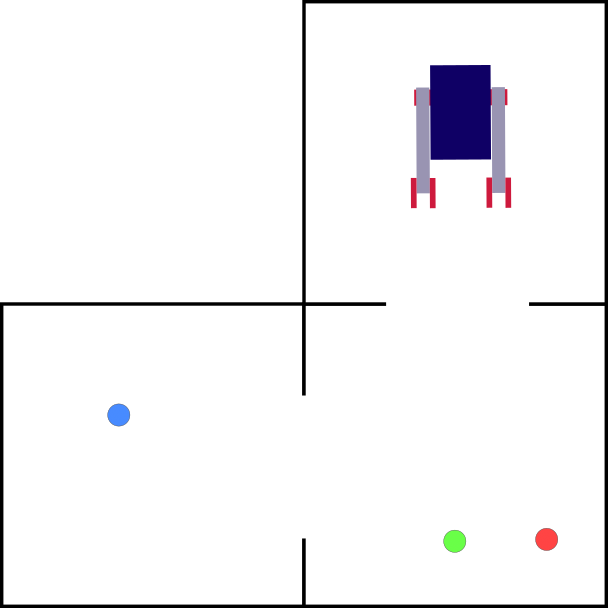
\includegraphics[width = 0.8\textwidth]{images/3_rooms/gd_3_0.png}
            \onslide<2>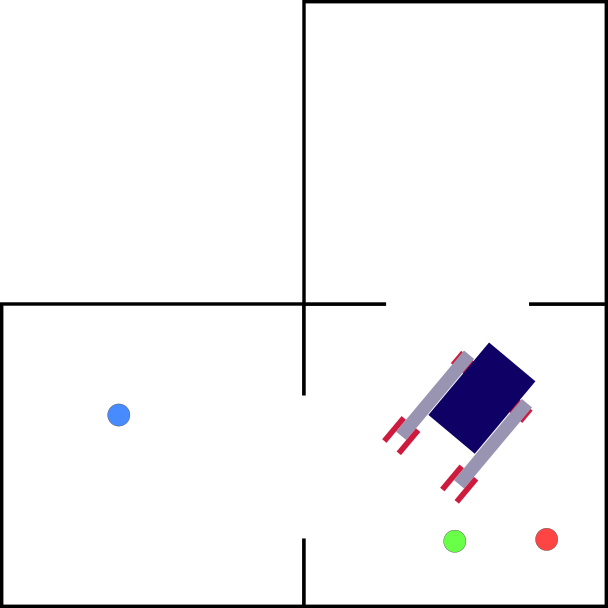
\includegraphics[width = 0.8\textwidth]{images/3_rooms/gd_3_1.png}
            \onslide<3>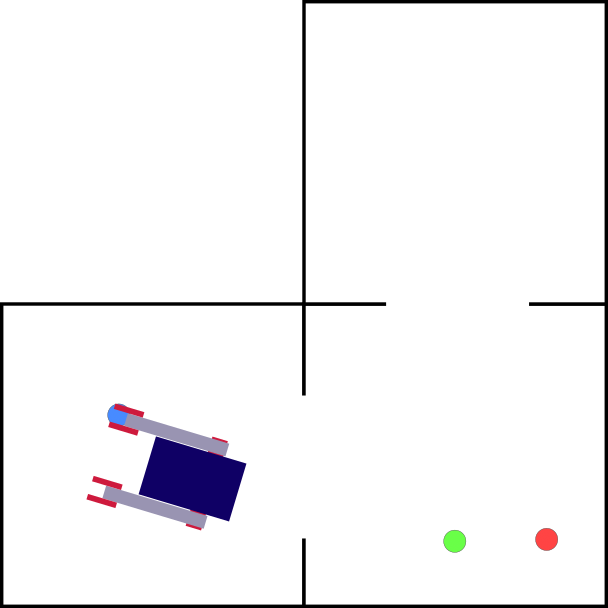
\includegraphics[width = 0.8\textwidth]{images/3_rooms/gd_3_3.png}
            \onslide<4->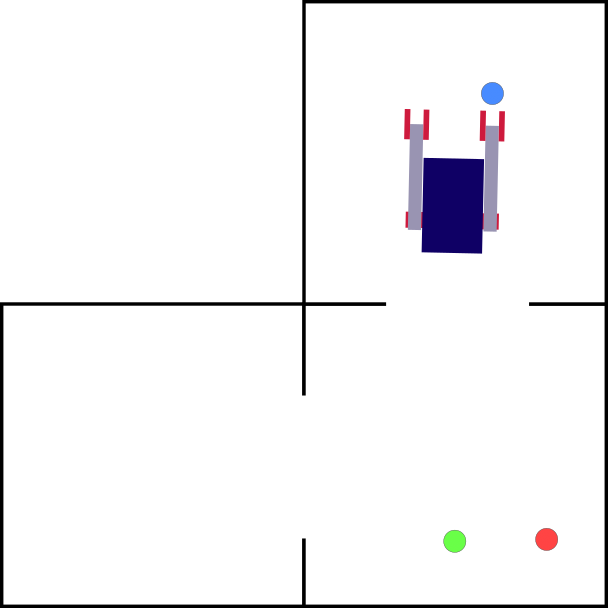
\includegraphics[width = 0.8\textwidth]{images/3_rooms/gd_3_6.png}
        \end{overprint}
    \end{column}
    \begin{column}<1->{0.5\textwidth}
        A \textit{robot} needs to place \textit{balls} in different \textit{rooms}
        \small
        \onslide<1->
        \begin{itemize}
            \item Actions:
            \onslide<2-> move
            \onslide<3->, pick
            \onslide<4-> , drop
            \onslide<5->
            \item State-functions:
                \begin{itemize}
                    \item at({ball, robot}) location
                    \item carry(?ball) gripper
                    \item connected
                \end{itemize}
            \item Tasks and methods: pick-and-drop(m1, m2), t\_move(m\_recursive, m\_already\_there)   
        \end{itemize}
    \end{column}
    
\end{columns} 
\end{frame}

\begin{frame}[c, fragile]{Problems of different sizes}
    \begin{columns}[c]
        \begin{column}[c]{0.3\textwidth}
            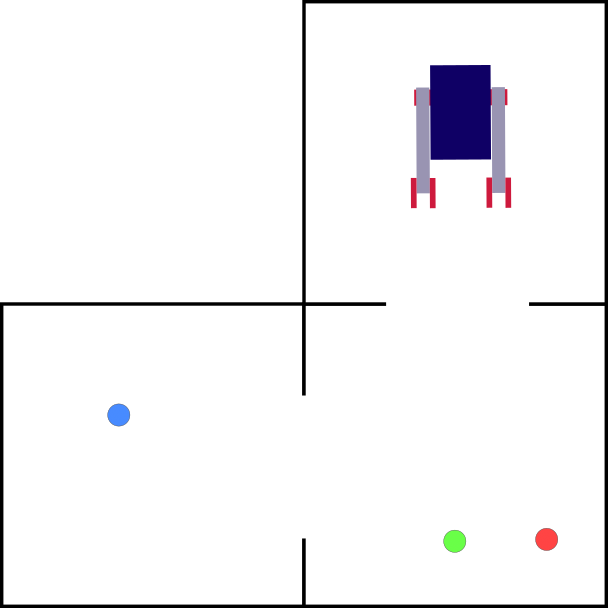
\includegraphics[width = 0.8\textwidth]{images/3_rooms/gd_3_0.png}
        \end{column}
        \begin{column}{0.1\textwidth}
            \centering $\rightarrow$
        \end{column}
        \begin{column}[c]{0.5\textwidth}
            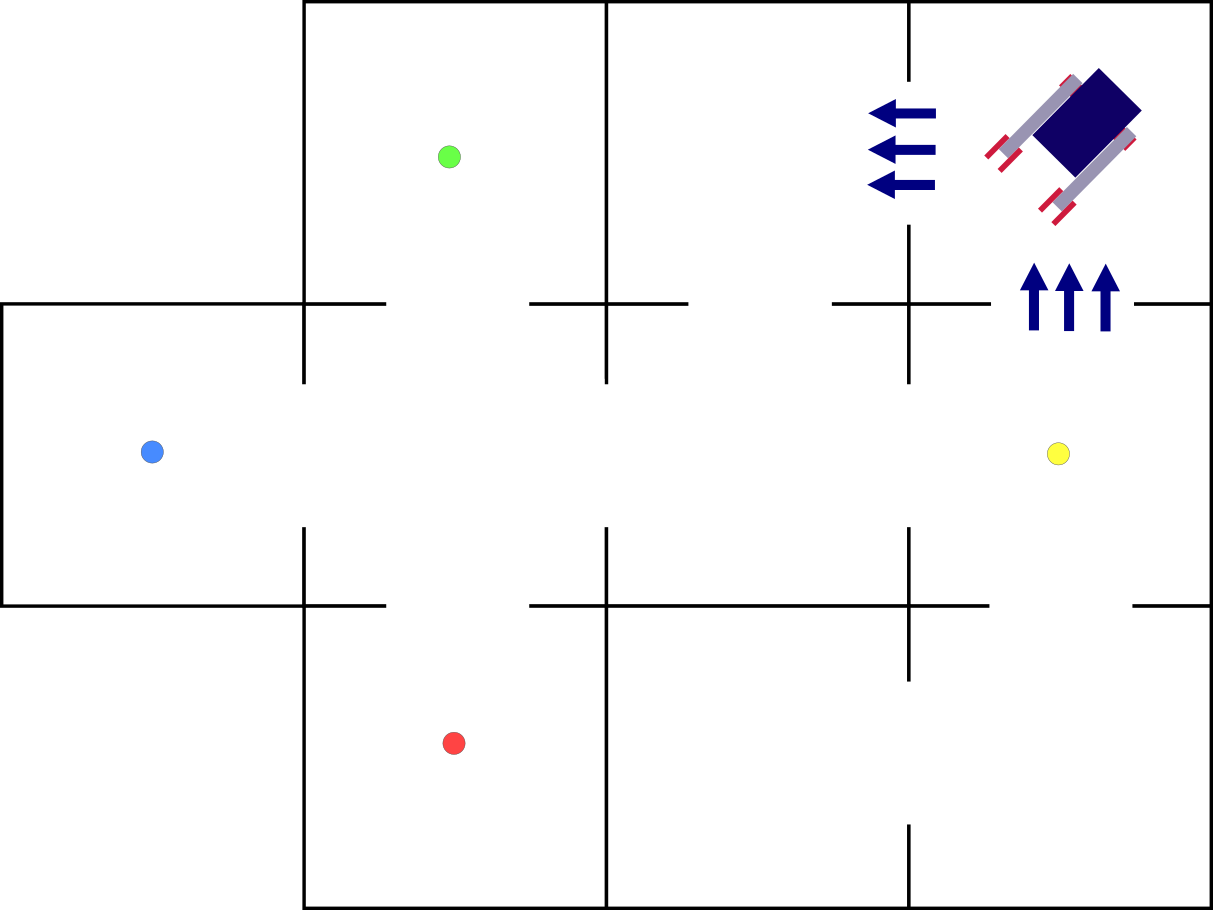
\includegraphics[width = \textwidth, angle=90]{images/11_rooms/gd_11_0.png}
        \end{column}
    \end{columns}
\end{frame}

\begin{frame}{Results}
  
\pgfplotstableread{datas/gripper_doors.dat}{\table}
\begin{columns}
    \begin{column}{0.45\textwidth}
        3 different Select:
        
        Greedy, Aries, Optimal Aries (Aries-opt)
    \end{column}

    \begin{column}{0.45\textwidth}
        Metrics in function of the number of room:
        \begin{itemize}
            \item Executed actions
            \item Total refinement time
        \end{itemize}
    \end{column}
\end{columns}

~

%Number of actions in functions of the number of rooms
\begin{columns}[T] % align columns
\begin{column}{.55\textwidth}

\begin{figure}[H]
    \caption{Executed actions}
    \begin{tikzpicture}
        \begin{axis}[
            legend image post style={scale=0.4},
        legend style={ at={(0.3,0.97)},anchor=north,legend cell align=left, font = \tiny},
            grid = both,
            minor tick num = 1,
            major grid style = {lightgray},
            minor grid style = {lightgray!25},
            width = \textwidth,
            %legend cell align = {left},
            %legend pos = north west
        ]
         
        \addplot[blue, ultra thick] table [x = {X}, y = {GA}] {\table};
         
        \addplot[red, ultra thick] table [x ={X}, y = {LA}] {\table};
        
        \addplot[green, ultra thick] table [x ={X}, y = {LOA}] {\table};       
        \legend{
            Greedy, 
            Aries,
            Aries-opt
        }
        
        
        \end{axis}
         
    \end{tikzpicture}
\end{figure}

\end{column}%
\begin{column}{.55\textwidth}
\begin{figure}
    \caption{Refinement time (s)}
\begin{tikzpicture}
    \begin{axis}[
        legend image post style={scale=0.4},
            legend style={at={(0.3,0.97)},anchor=north,legend cell align=left, font = \tiny},
            grid = both,
            minor tick num = 1,
            major grid style = {lightgray},
            minor grid style = {lightgray!25},
            width = \textwidth,
            %legend cell align = {left},
            %legend pos = north west
        ]
            
        \addplot[blue, ultra thick] table [x = {X}, y = {GT}] {\table};
        \addlegendentry{Greedy}
            
        \addplot[red, ultra thick] table [x ={X}, y = {LT}] {\table};
        \addlegendentry{Aries}
        
        \addplot[green, ultra thick] table [x ={X}, y = {LOT}] {\table};
        \addlegendentry{Aries-opt}
    
    \end{axis}
\end{tikzpicture} 
\end{figure}

\end{column}%
\end{columns}  
\end{frame}




